\documentclass{cmc}
\usepackage{listings}
\usepackage{makecell}
\begin{document}

\pagestyle{fancy}
\lhead{\textit{\textbf{Computational Motor Control, Spring 2022} \\
    Final project, Lab 6, NOT GRADED}} \rhead{Student \\ Names}

\section*{Student names: \ldots (please update)}

\textit{\textbf{Instructions:} This week, you will be installing and testing the
  simulation environment that you will be using for the final project. Make sure
  to install it as soon as possible and get help from the TAs if you encounter
  any issues before you officially start the project next week.}

\subsection*{Simulation environment installation}

The installation of the simulation environment can be completed using a script
found in the Lab6 folder. You can run it by simply calling:

\label{sec:mujoco-inst}
\begin{lstlisting}[language=Bash]
  >> python setup_sim_env.py
\end{lstlisting}

This will install the \textit{MuJoCo} simulator and the \textit{dm\_control}
package which are software maintained by Deepmind for running robot
simulations. It will also install the \textit{farms\_core},
\textit{farms\_mujoco} and \textit{farms\_sim} packages developed at the
Biorobotics Laboratory (BioRob). If you are interested in knowing more about
\textit{MuJoCo}, you can find out more on \href{https://mujoco.org/}{\corr{the
    official website}}.

\corr{\textit{IMPORTANT:}} Make sure you have activated and are using your
virtual environment and its python interpreter that that you have created for
this course.

\corr{\textit{NOTE:}} If you are unclear about the basic steps then refer back
to Lab 0 documentation here
\href{https://farmsim.gitlab.io/courses/cmc-2022/}{\corr{cmc-installation-help}}


\subsection*{Examples}
We have provided an example based on next week's project to get you accustomed
to the MuJoCo graphical interface. You can try running it by calling:

\label{sec:mujoco-example}
\begin{lstlisting}[language=Bash]
  >> python example.py
\end{lstlisting}

This script is available under Lab6/Python.

\subsubsection*{Graphical User Interface Interaction}
When you run the example script, a Graphical User Interface (GUI) should launch,
like the one shown in Figure \ref{fig:mujoco-gui}

You can use the left mouse click to move around the scene and right mouse click
to rotate the camera. You can also select a part of the robot by double left
clicking on a part. Once selected, you can then interact with it by holding the
CONTROL key and dragging with left or right click. Try it out for yourself to
familiarise with the interface.

There are many keyboard shortcuts also available

\begin{itemize}
\item Press SPACE to toggle play/pause
\item Press ``\textquotesingle'' / ``\textsuperscript{$\wedge$}'' to change
  speed factor (between zero (0) and backspace)
\item Press w to toggle wireframe
\item Press t to toggle transparency
\item Press s to toggle shadows
\item Press c to show collisions
\item Press f to show collisions forces, combine with p to show
  friction/reaction
\item Press b to show external forces (try in water later on)
\item And many more...
\end{itemize}

\begin{figure}[H]
  \centering 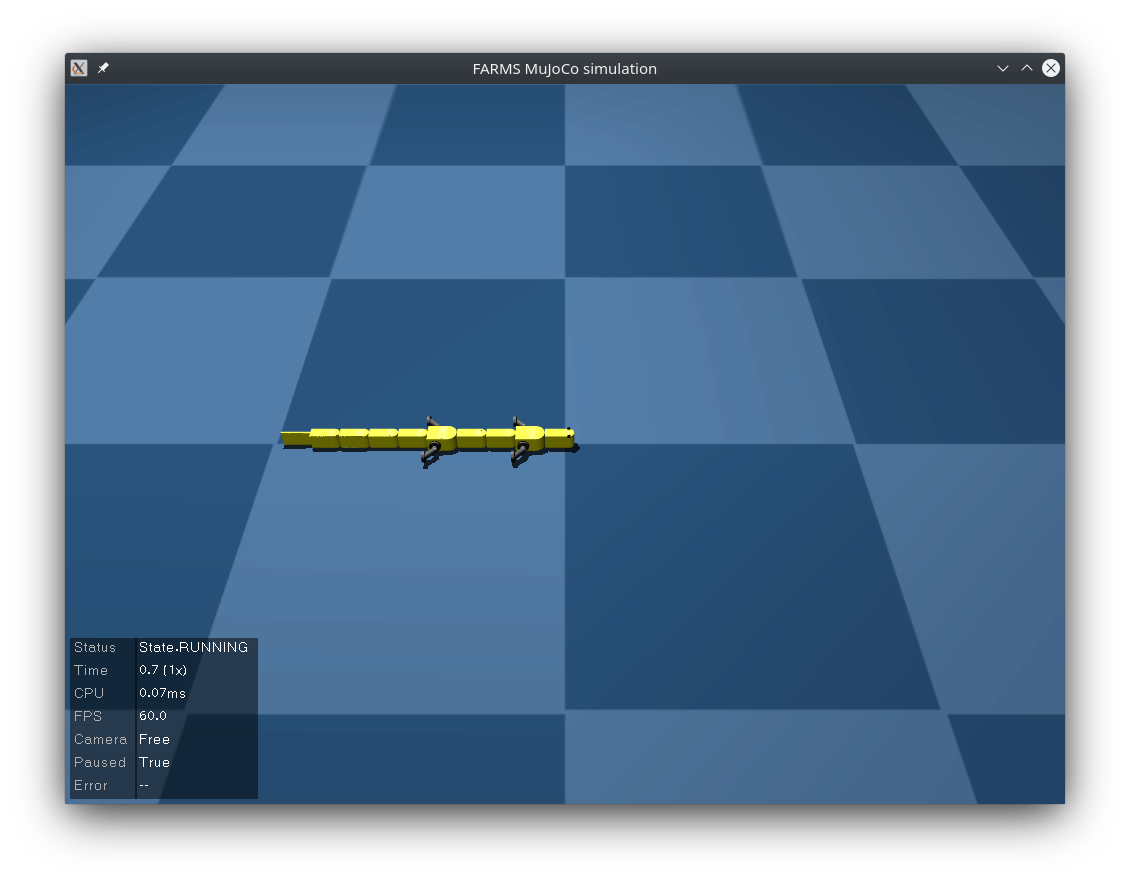
\includegraphics[width=\textwidth]{figures/mujoco-gui}
  \caption{MuJoCo/dm\_control Graphical User Interface}
  \label{fig:mujoco-gui}
\end{figure}

\textbf{Important things to explore with the provided example}
\begin{itemize}
\item Changing the view of the scene using the controls above
\item Interaction with the objects in the scene
\item Try changing to a water arena in the example script and showing the forces
  acting on the body (b)
\end{itemize}

\subsection*{Preparing for the project}

Once you are done with the installation and have tried the simulation
environment. The best way to prepare for the upcoming project is to read the two
following paper in detail:

\begin{itemize}
\item \href{https://www.science.org/doi/10.1126/science.1138353}{Ijspeert, Auke Jan, et al. "From swimming to walking with a salamander robot driven by a spinal cord model." science 315.5817 (2007): 1416-1420.}
\item \href{https://www.science.org/doi/10.1126/scirobotics.abf6354}{Thandiackal, Robin, et al. "Emergence of robust self-organized undulatory swimming based on local hydrodynamic force sensing." Science Robotics 6.57 (2021): eabf6354.}
\end{itemize}

\begin{center}
  Happy reading!
\end{center}

\end{document}

%%% Local Variables:
%%% mode: latex
%%% TeX-master: t
%%% End: